\section{Preliminaries: Defining the Geosodic Tree}
\label{sec:prelim}

We now define the \emph{Geosodic Tree}, a structure that grows by 
``pivot + fully formed right subtree'' steps at each depth, 
thus remaining \emph{meltdown-free}: 
no pre-existing node is ever re-labeled or partially altered when moving 
from depth $d$ to $d+1$. The result is a \emph{perfectly balanced} tree 
at each level, eventually labeled in-order upon completion.

\subsection{Construction at Each Depth}
\label{subsec:construction}

At \emph{depth} $0$, we begin with a single node $r$ (the root). To go from a Geosodic Tree
of depth $d$ to depth $d+1$, we do the following:

\begin{enumerate}
  \item \textbf{Add a new pivot node as the root,} making the old depth-$d$ tree its left subtree.
  \item \textbf{Attach a perfect right subtree of depth $d$}, which has $2^{d+1}-1$ nodes,
        plus the pivot (1 node) added in Step~1, for a total of $2^{d+1}$ new nodes.
\end{enumerate}

Since a perfect binary tree of depth $d$ contains $2^{d+1}-1$ nodes, 
adding one such subtree on the right (and the new pivot) yields exactly $2^{d+1}$ new nodes 
when advancing from depth $d$ to $d+1$. 

\paragraph{Resulting Node Count.}
If the old tree (at depth $d$) had $2^{d+1}-1$ total nodes, adding these $2^{d+1}$ new nodes 
brings the total to
\[
  \bigl(2^{d+1}-1\bigr) + 2^{d+1} 
  \;=\;
  2^{d+2}-1,
\]
which is precisely a perfect binary tree of depth $d+1$. Once this new level is fully assembled,
we label the resulting tree \emph{in-order}, though we do \emph{not} perform any 
key-based insertions as in BSTs.

\begin{figure}[ht]
  \centering
  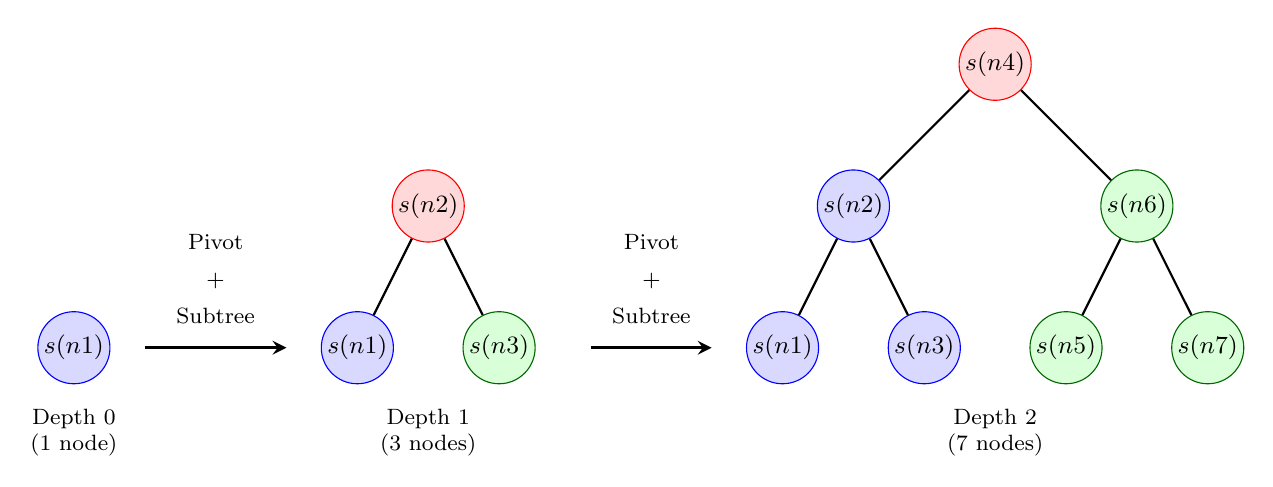
\begin{tikzpicture}[
      scale=.9,
      % The actual tree nodes:
      every node/.style={circle, draw, minimum size=6.5mm, inner sep=1pt, font=\small},
      old/.style={draw=blue, fill=blue!15},
      pivot/.style={draw=red, fill=red!15},
      new/.style={draw=green!40!black, fill=green!15},
      thickedge/.style={draw, thick},
      >=stealth,
      baseline={(current bounding box.south)} % align figure along the bottom
  ]
  
  %%%%%%%%%%%%%%%%%%%%%%%%%%%%%%%%%%%%%%%%%%%%%%%%%%%%%%%%
  % (1) DEPTH=1 => Single node s(n1)
  %%%%%%%%%%%%%%%%%%%%%%%%%%%%%%%%%%%%%%%%%%%%%%%%%%%%%%%%
  \node[old] (A1) at (0,0) {$s(n1)$};
  
  % Depth label below, two lines:
  \node[
    draw=none, fill=none, shape=rectangle, 
    font=\footnotesize, align=center
  ] 
  at (0,-1.2) {Depth 0\\(1 node)};
  
  %%%%%%%%%%%%%%%%%%%%%%%%%%%%%%%%%%%%%%%%%%%%%%%%%%%%%%%%
  % ARROW from first to second
  %%%%%%%%%%%%%%%%%%%%%%%%%%%%%%%%%%%%%%%%%%%%%%%%%%%%%%%%
  \draw[->, very thick] 
    (1,0) -- (3,0)
    node[midway,above=7pt,draw=none,fill=none,shape=rectangle,font=\footnotesize,align=center]
         {Pivot\\[4pt]+\\[4pt]Subtree};
  
  %%%%%%%%%%%%%%%%%%%%%%%%%%%%%%%%%%%%%%%%%%%%%%%%%%%%%%%%
  % (2) DEPTH=2 => 3 nodes total
  %%%%%%%%%%%%%%%%%%%%%%%%%%%%%%%%%%%%%%%%%%%%%%%%%%%%%%%%
  % We'll put old node s(n1) at x=4,y=0
  % pivot s(n2) at x=4,y=2  (2 units above old node)
  % new node s(n3) at x=6,y=0
  
  \node[old]   (Bleft) at (4,0)   {$s(n1)$};
  \node[pivot] (Broot) at (5,2)   {$s(n2)$};
  \draw[thickedge] (Broot) -- (Bleft);
  
  \node[new]   (Bright) at (6,0)  {$s(n3)$};
  \draw[thickedge] (Broot) -- (Bright);
  
  % Depth label below
  \node[
    draw=none, fill=none, shape=rectangle, font=\footnotesize, align=center
  ] 
  at (5,-1.2) {Depth 1\\(3 nodes)};
  
  %%%%%%%%%%%%%%%%%%%%%%%%%%%%%%%%%%%%%%%%%%%%%%%%%%%%%%%%
  % ARROW from second to third
  %%%%%%%%%%%%%%%%%%%%%%%%%%%%%%%%%%%%%%%%%%%%%%%%%%%%%%%%
  \draw[->, very thick]
    (7.3,0) -- (9.0,0)
    node[midway,above=7pt,draw=none,fill=none,shape=rectangle,font=\footnotesize,align=center]
         {Pivot\\[4pt]+\\[4pt]Subtree};
  
  %%%%%%%%%%%%%%%%%%%%%%%%%%%%%%%%%%%%%%%%%%%%%%%%%%%%%%%%
  % (3) DEPTH=3 => 7 nodes total
  %%%%%%%%%%%%%%%%%%%%%%%%%%%%%%%%%%%%%%%%%%%%%%%%%%%%%%%%
  % We'll keep old node s(n1) at (10,0)
  % old pivot s(n2) at (10,2)
  % new pivot s(n4) at (10,4)
  % old right node s(n3) at (12,0)
  % new subtree root s(n5) at (12,2)
  % leaves s(n6) at (11.5,0) and s(n7) at (12.5,0)
  
  \node[old]   (ColdLeft)  at (10,0) {$s(n1)$};
  \node[old]   (ColdRoot)  at (11,2) {$s(n2)$};
  \draw[thickedge] (ColdRoot) -- (ColdLeft);
  
  \node[pivot] (Croot)     at (13,4) {$s(n4)$};
  \draw[thickedge] (Croot) -- (ColdRoot);
  
  \node[old]   (ColdRight) at (12,0) {$s(n3)$};
  \draw[thickedge] (ColdRoot) -- (ColdRight);
  
  \node[new]   (CrightRoot) at (15,2) {$s(n6)$};
  \draw[thickedge] (Croot) -- (CrightRoot);
  
  \node[new]   (CrightL)   at (14,0) {$s(n5)$};
  \node[new]   (CrightR)   at (16,0) {$s(n7)$};
  
  \draw[thickedge] (CrightRoot) -- (CrightL);
  \draw[thickedge] (CrightRoot) -- (CrightR);
  
  % Depth label for third tree, two lines
  \node[
    draw=none, fill=none, shape=rectangle,
    font=\footnotesize, align=center
  ] 
  at (13,-1.2) {Depth 2\\(7 nodes)};
  
  \end{tikzpicture}
  
  \caption{From left (Depth 0) to right (Depth 2), illustrating meltdown-free expansions:
  old nodes (blue) at the bottom, pivot node(s) (red) placed above,
  and any new subtree nodes (green) at the bottom again. 
  We space each depth label on two lines below the tree, 
  and put line breaks in the arrow labels as well.}
  \label{fig:geosodic-expansion}
  \end{figure}
  

\begin{definition}[Geosodic Tree]
\label{def:geosodic-tree}
A \emph{Geosodic Tree} of depth $d$ is a rooted binary tree with $2^{d+1}-1$ nodes,
obtained by starting at a single node (depth~0) and, for each level $k=0,1,\dots,d-1$, 
adding exactly $2^{k+1}$ new nodes (one pivot plus a perfect right subtree of depth $k$) 
to form depth $k+1$. Throughout, no re-labeling or partial reshuffling of old nodes occurs,
keeping each expansion \emph{meltdown-free}. The final tree at depth $d$ is \emph{perfect} 
(all leaves at level $d$), \emph{in-order labeled} once assembled, and remains 
\emph{meltdown-free} at every stage.
\end{definition}

These steps guarantee:
\begin{itemize}
  \item \textbf{Perfect Balance:} Every depth-$d$ tree is a complete binary tree of size $2^{d+1}-1$.
  \item \textbf{No Partial Insertions:} Each step adds a full subtree of depth $d$ (plus pivot) 
        rather than single-node insertions.
  \item \textbf{No Re-labeling (Meltdown-Free):} Old nodes from level $d$ stay intact; 
        expansions attach only \emph{new} nodes.
\end{itemize}

\subsection{No Smaller Step Than Doubling}
\label{subsec:no-smaller}

We justify why one \emph{cannot} add fewer than $2^{d+1}$ new nodes (counting the pivot) 
when moving from depth $d$ to $d+1$ without violating the geosodic (meltdown-free) properties:

\begin{lemma}[No Smaller Step than Doubling]
\label{lem:no-smaller-step}
Let $G_d$ be a Geosodic Tree of depth $d$, which has $2^{d+1}-1$ total nodes 
and is perfectly balanced. Suppose we attempt to form a depth-$(d+1)$ tree by adding 
fewer than $2^{d+1}$ new nodes in one expansion step. Then either:
\begin{enumerate}
  \item The resulting tree is \emph{not} a perfect binary tree at depth $d+1$, or
  \item A local restructure (partial rotation, re-labeling, etc.) is needed to fill 
        or shift nodes, contradicting the meltdown-free principle.
\end{enumerate}
Hence, the only way to achieve a depth-$(d+1)$ Geosodic Tree from $G_d$ while preserving 
perfect balance and no re-labeling is to add exactly $2^{d+1}$ new nodes (one pivot plus a 
fully formed right subtree of depth $d$). In \S\ref{subsec:uniqueness},
we will prove this condition uniquely forces the Geosodic Tree structure
at each depth, making it \emph{canonical} among meltdown-free expansions.

\begin{proof}[Proof Sketch]
A perfect binary tree of depth $d$ has $2^{d+1}-1$ nodes; 
one of depth $d+1$ must have $2^{(d+1)+1}-1 = 2^{d+2}-1$. 
Thus, the gap in node count is 
\[
  \bigl(2^{d+2}-1\bigr) - \bigl(2^{d+1}-1\bigr) 
  \;=\;
  2^{d+1}.
\]
If fewer than $2^{d+1}$ new nodes are introduced, the resulting structure 
cannot reach $2^{d+2}-1$ total nodes at depth $d+1$ without either:
\begin{itemize}
  \item Becoming imperfect (missing leaves), or
  \item Re-labeling or reshuffling older nodes to fill gaps, breaking meltdown-free increments.
\end{itemize}
Therefore, the minimal and \emph{unique} meltdown-free expansion consistent with 
perfect balance is adding $2^{d+1}$ new nodes in one shot: 
one pivot plus a perfect right subtree of depth $d$ (which contains $2^{d+1}-1$ nodes).
\end{proof}
\end{lemma}

\subsection{Distinction from Classic Binary Search Trees}
\label{sec:distinction}

Readers familiar with \emph{binary search trees} (BSTs) may wonder if Geosodic Trees 
are merely a variant of \emph{balanced BSTs} (e.g.\ AVL or Red--Black Trees~\cite{Cormen2009}). 
While both are “binary trees” and can use an in-order labeling, 
the Geosodic Tree differs fundamentally in its construction and objective:

\begin{itemize}
    \item \textbf{No Local Re-balancing.}
    In a self-balancing BST (AVL, Red--Black, etc.), each node insertion 
    can trigger rotations, effectively “re-labeling” subtrees or changing parent-child links 
    to maintain height bounds. By contrast, the Geosodic Tree has \emph{no rotations or partial fixes}. 
    We add a pivot node plus an entire right subtree \emph{at once}, leaving older nodes undisturbed.

    \item \textbf{Minimal, Meltdown-Free Expansions.}
    BSTs typically support node-by-node insertion. 
    Our Geosodic Tree \emph{doubles} at each depth—the minimal meltdown-free step 
    that keeps balance and forbids partial expansions or re-labeling. 
    Hence, old labels remain stable, which standard BSTs do not guarantee.

    \item \textbf{Different “Ordered” Notion.}
    A normal BST enforces 
    \(\text{(left subtree values)} < \text{(node value)} < \text{(right subtree values)}\). 
    Here, “ordered” means an \emph{in-order labeling} \emph{after} the depth is fully built, 
    not a key-based ordering \emph{during} insertion.

    \item \textbf{Focus on Enumeration, Not Searching.}
    Traditional BSTs aim for efficient lookups. 
    Our Geosodic Tree aims for \emph{universal enumeration} and meltdown-free expansions:
    each new depth encloses all prior nodes plus a fully formed subtree, 
    staying perfectly balanced. Searching is incidental—our main results concern 
    meltdown-free increments and code embeddings, not operational performance.
\end{itemize}

Thus, while the Geosodic Tree and BSTs both have in-order traversals, 
they embody \emph{very} different growth principles: local rebalancing or partial insertions 
in BSTs, versus whole-subtree expansions in meltdown-free steps for Geosodic Trees.

\subsection{DAG Interpretation}

Although we call it a “tree,” one can view a Geosodic Tree as a \emph{directed acyclic graph (DAG)} 
rooted at the initial node. Each depth adds fresh nodes and edges in a strictly forward direction 
(from pivot to newly created subtrees). No rearrangement of older edges occurs, preventing cycles 
or rewiring. Thus, each node has a unique parent (except the root), and there is exactly 
one directed path from the root to any node. 

This DAG viewpoint further underscores that meltdown-free expansions never alter existing labels 
or edges—every new depth is just appended, keeping a strict partial order of creation.

\subsection{Auxiliary Labels}

In some proofs, we assign temporary “auxiliary” labels (e.g., 0/1 for left/right paths, 
or numeric indexing for partial sums). Such \emph{auxiliary} labels do \emph{not} alter 
the tree’s meltdown-free property—old node identities remain intact, and no re-labeling occurs. 
These labels are solely for analysis (like referencing paths), consistent with 
the “no partial expansions” principle.

\begin{figure}[H]
    \centering
    \scalebox{0.7}{%
    \begin{tikzpicture}[
      old/.style={draw=blue, fill=blue!15, circle, minimum size=7mm, inner sep=1pt, font=\small},
      pivot/.style={draw=red, fill=red!15, circle, minimum size=7mm, inner sep=1pt, font=\small},
      new/.style={draw=green!40!black, fill=green!15, circle, minimum size=7mm, inner sep=1pt, font=\small},
      every path/.style={thick},
      xscale=1.1, yscale=1.1,
      level distance=1.5cm, sibling distance=2cm,
      >=stealth,
    ]
    
    % --------------------------------------------------------------------
    % We draw exactly ONE depth-3 Geosodic Tree shape, color-coded:
    %  - The "old" depth-2 subtree on the left (blue)
    %  - The new pivot node at the top (red)
    %  - The new right subtree of depth-2 (green)
    %
    % Then we replicate that shape 3 times vertically,
    % just changing the *labels* on each copy.
    
    % Node counts total = 15 for depth-3:
    %  - Depth-2 subtree has 7 old nodes
    %  - 1 pivot node
    %  - Another depth-2 subtree has 7 new nodes
    
    %%%%%%%%%%%%%%%%%%%%%%%%%%%%%%%%%%%%%%%%%%%%%%%%
    % ============== FIRST ROW (1..15 in in-order) =
    %%%%%%%%%%%%%%%%%%%%%%%%%%%%%%%%%%%%%%%%%%%%%%%%
    \def\Yshift{0}
    
    % Left subtree (OLD, depth=2)
    \node[old] (OL)   at (-4, \Yshift - 1.0) {}; 
    \node[old] (OLL)  at (-6, \Yshift - 2.8) {};
    \node[old] (OLR)  at (-2, \Yshift - 2.8) {};
    \node[old] (OLLL) at (-7, \Yshift - 4.5) {};
    \node[old] (OLLR) at (-5, \Yshift - 4.5) {};
    \node[old] (OLRL) at (-3, \Yshift - 4.5) {};
    \node[old] (OLRR) at (-1, \Yshift - 4.5) {};
    
    % Pivot (RED)
    \node[pivot] (PIV) at (0, \Yshift + 0.5) {};
    
    % Right subtree (NEW, depth=2)
    \node[new] (NR)   at ( 4, \Yshift - 1.0) {}; 
    \node[new] (NRL)  at ( 2, \Yshift - 2.8) {}; % left child
    \node[new] (NRR)  at ( 6, \Yshift - 2.8) {}; % right child
    \node[new] (NRLL) at ( 1, \Yshift - 4.5) {};
    \node[new] (NRLR) at ( 3, \Yshift - 4.5) {};
    \node[new] (NRRL) at ( 5, \Yshift - 4.5) {};
    \node[new] (NRRR) at ( 7, \Yshift - 4.5) {};
    
    % Edges
    \draw (PIV) -- (OL);
    \draw (PIV) -- (NR);
    
    \draw (OL) -- (OLL);
    \draw (OL) -- (OLR);
    \draw (OLL) -- (OLLL);
    \draw (OLL) -- (OLLR);
    \draw (OLR) -- (OLRL);
    \draw (OLR) -- (OLRR);
    
    \draw (NR) -- (NRL);
    \draw (NR) -- (NRR);
    \draw (NRL) -- (NRLL);
    \draw (NRL) -- (NRLR);
    \draw (NRR) -- (NRRL);
    \draw (NRR) -- (NRRR);
    
    % In-order labeling: 
    % Left subtree: OLLL->1, OLL->2, OLLR->3, OL->4, OLRL->5, OLR->6, OLRR->7
    % Pivot -> 8
    % Right subtree: NRLL->9, NRL->10, NRLR->11, NR->12, NRRL->13, NRR->14, NRRR->15
    \node[old]   at (OLLL) {1};
    \node[old]   at (OLL)  {2};
    \node[old]   at (OLLR) {3};
    \node[old]   at (OL)   {4};
    \node[old]   at (OLRL) {5};
    \node[old]   at (OLR)  {6};
    \node[old]   at (OLRR) {7};
    
    \node[pivot] at (PIV)  {8};
    
    \node[new]   at (NRLL) {9};
    \node[new]   at (NRL)  {10};
    \node[new]   at (NRLR) {11};
    \node[new]   at (NR)   {12};
    \node[new]   at (NRRL) {13};
    \node[new]   at (NRR)  {14};
    \node[new]   at (NRRR) {15};
    
    \node[draw=none,fill=none,font=\bfseries]
          at (0, \Yshift + 1.6)
          {Depth-3 Geosodic Tree --- In-order $\{1,\dots,15\}$};
    
    
    %%%%%%%%%%%%%%%%%%%%%%%%%%%%%%%%%%%%%%%%%%%%%%%%%%%%%%%%%%%%%%%%%%%%
    % ===== SECOND ROW (fractions n/2^{n-1} or n/16 for d=3) ===========
    %%%%%%%%%%%%%%%%%%%%%%%%%%%%%%%%%%%%%%%%%%%%%%%%%%%%%%%%%%%%%%%%%%%%
    \def\Yshift{-8}
    
    % Repeat the same shape (old/pivot/new) with a Y offset:
    \node[old] (OL2)   at (-4, \Yshift - 1.0) {};
    \node[old] (OLL2)  at (-6, \Yshift - 2.8) {};
    \node[old] (OLR2)  at (-2, \Yshift - 2.8) {};
    \node[old] (OLLL2) at (-7, \Yshift - 4.5) {};
    \node[old] (OLLR2) at (-5, \Yshift - 4.5) {};
    \node[old] (OLRL2) at (-3, \Yshift - 4.5) {};
    \node[old] (OLRR2) at (-1, \Yshift - 4.5) {};
    
    \node[pivot] (PIV2) at (0, \Yshift + 0.5) {};
    
    \node[new] (NR2)   at ( 4, \Yshift - 1.0) {};
    \node[new] (NRL2)  at ( 2, \Yshift - 2.8) {};
    \node[new] (NRR2)  at ( 6, \Yshift - 2.8) {};
    \node[new] (NRLL2) at ( 1, \Yshift - 4.5) {};
    \node[new] (NRLR2) at ( 3, \Yshift - 4.5) {};
    \node[new] (NRRL2) at ( 5, \Yshift - 4.5) {};
    \node[new] (NRRR2) at ( 7, \Yshift - 4.5) {};
    
    % Edges
    \draw (PIV2) -- (OL2);
    \draw (PIV2) -- (NR2);
    
    \draw (OL2) -- (OLL2);
    \draw (OL2) -- (OLR2);
    \draw (OLL2) -- (OLLL2);
    \draw (OLL2) -- (OLLR2);
    \draw (OLR2) -- (OLRL2);
    \draw (OLR2) -- (OLRR2);
    
    \draw (NR2) -- (NRL2);
    \draw (NR2) -- (NRR2);
    \draw (NRL2) -- (NRLL2);
    \draw (NRL2) -- (NRLR2);
    \draw (NRR2) -- (NRRL2);
    \draw (NRR2) -- (NRRR2);
    
    % In-order fractional labels: ( n/16 for n=1..15 )
    \node[old]   at (OLLL2) {$\tfrac{1}{16}$};
    \node[old]   at (OLL2)  {$\tfrac{2}{16}$};
    \node[old]   at (OLLR2) {$\tfrac{3}{16}$};
    \node[old]   at (OL2)   {$\tfrac{4}{16}$};
    \node[old]   at (OLRL2) {$\tfrac{5}{16}$};
    \node[old]   at (OLR2)  {$\tfrac{6}{16}$};
    \node[old]   at (OLRR2) {$\tfrac{7}{16}$};
    
    \node[pivot] at (PIV2) {$\tfrac{8}{16}$};
    
    \node[new]   at (NRLL2) {$\tfrac{9}{16}$};
    \node[new]   at (NRL2)  {$\tfrac{10}{16}$};
    \node[new]   at (NRLR2) {$\tfrac{11}{16}$};
    \node[new]   at (NR2)   {$\tfrac{12}{16}$};
    \node[new]   at (NRRL2) {$\tfrac{13}{16}$};
    \node[new]   at (NRR2)  {$\tfrac{14}{16}$};
    \node[new]   at (NRRR2) {$\tfrac{15}{16}$};
    
    \node[draw=none,fill=none,font=\bfseries]
          at (0, \Yshift + 1.6)
          {Depth-3 --- Labels $n/2^{d+1}$ (viewing $d=3$)};
    
    
    %%%%%%%%%%%%%%%%%%%%%%%%%%%%%%%%%%%%%%%%%%%%%%%%%%%%%%%%%%%%%%%%%%%%
    % =========== THIRD ROW (4-bit binary 0001..1111) ==================
    %%%%%%%%%%%%%%%%%%%%%%%%%%%%%%%%%%%%%%%%%%%%%%%%%%%%%%%%%%%%%%%%%%%%
    \def\Yshift{-16}
    
    \node[old] (OL3)   at (-4, \Yshift - 1.0) {};
    \node[old] (OLL3)  at (-6, \Yshift - 2.8) {};
    \node[old] (OLR3)  at (-2, \Yshift - 2.8) {};
    \node[old] (OLLL3) at (-7, \Yshift - 4.5) {};
    \node[old] (OLLR3) at (-5, \Yshift - 4.5) {};
    \node[old] (OLRL3) at (-3, \Yshift - 4.5) {};
    \node[old] (OLRR3) at (-1, \Yshift - 4.5) {};
    
    \node[pivot] (PIV3) at (0, \Yshift + 0.5) {};
    
    \node[new] (NR3)   at ( 4, \Yshift - 1.0) {};
    \node[new] (NRL3)  at ( 2, \Yshift - 2.8) {};
    \node[new] (NRR3)  at ( 6, \Yshift - 2.8) {};
    \node[new] (NRLL3) at ( 1, \Yshift - 4.5) {};
    \node[new] (NRLR3) at ( 3, \Yshift - 4.5) {};
    \node[new] (NRRL3) at ( 5, \Yshift - 4.5) {};
    \node[new] (NRRR3) at ( 7, \Yshift - 4.5) {};
    
    % Edges
    \draw (PIV3) -- (OL3);
    \draw (PIV3) -- (NR3);
    
    \draw (OL3) -- (OLL3);
    \draw (OL3) -- (OLR3);
    \draw (OLL3) -- (OLLR3);
    \draw (OLL3) -- (OLLL3);
    \draw (OLR3) -- (OLRL3);
    \draw (OLR3) -- (OLRR3);
    
    \draw (NR3) -- (NRL3);
    \draw (NR3) -- (NRR3);
    \draw (NRL3) -- (NRLL3);
    \draw (NRL3) -- (NRLR3);
    \draw (NRR3) -- (NRRL3);
    \draw (NRR3) -- (NRRR3);
    
    % In-order binary: from 0001..1111
    \node[old]   at (OLLL3) {0001};
    \node[old]   at (OLL3)  {0010};
    \node[old]   at (OLLR3) {0011};
    \node[old]   at (OL3)   {0100};
    \node[old]   at (OLRL3) {0101};
    \node[old]   at (OLR3)  {0110};
    \node[old]   at (OLRR3) {0111};
    
    \node[pivot] at (PIV3) {1000};
    
    \node[new]   at (NRLL3) {1001};
    \node[new]   at (NRL3)  {1010};
    \node[new]   at (NRLR3) {1011};
    \node[new]   at (NR3)   {1100};
    \node[new]   at (NRRL3) {1101};
    \node[new]   at (NRR3)  {1110};
    \node[new]   at (NRRR3) {1111};
    
    \node[draw=none,fill=none,font=\bfseries]
          at (0, \Yshift + 1.6)
          {Depth-3 --- Binary labels `0001`--`1111`};
    
    \end{tikzpicture}
    } % end scalebox
    \caption{A single Geosodic Tree at depth 3 (15 nodes) with three different 
    “auxiliary” labelings. Top: natural numbers 1--15 in proper in-order. 
    Middle: fractional labels \(\tfrac{n}{16}\) for \(n=1\ldots15\) -- at each pivot, we decide whether to add or subtract 
    \(\tfrac{1}{16}\) according to left or right and create a partial sum that approximates any real [0,1] to an arbitrary precision depth d. 
    Bottom: 4-bit binary from `0001` to `1111`. 
    In each drawing, the \textcolor{blue}{old depth-2 nodes} remain, the 
    \textcolor{red}{pivot node} is newly placed, and the 
    \textcolor{green!30!black}{new} depth-2 subtree is attached on the right, 
    illustrating meltdown-free expansion from depth 2 to depth 3.}
    \label{fig:depth3-alt-labels}
    \end{figure}
     